\documentclass[aspectratio=169]{beamer}
\usepackage{FAU-beamer}
\usepackage[ngerman,english]{babel}
\usepackage{xcolor}
\usepackage{amsmath}
\usepackage{amsfonts}
\usepackage{amssymb}
\usepackage{euler}
\usepackage{etoolbox}
\usepackage{pgfplots}
\usepackage{tikz}
\usepackage{enumitem}
\usepackage{mathtools}
\usepackage[rm={lining,proportional},sf={lining,proportional},tt={lining,tabular,monowidth}]{cfr-lm}
\usepgfplotslibrary{patchplots}
\usetikzlibrary{patterns, positioning, arrows, fadings}
\tikzfading[name=fade out, inner color=transparent!0, outer color=transparent!100]
\usepackage[
bibstyle=authoryear,
citestyle=authoryear,
maxcitenames=2,
maxbibnames=100,
backend=bibtex
]{biblatex}
\usepgfplotslibrary{external} 
\tikzexternalize
\hypersetup{
    unicode=true,
    pdfencoding=unicode,
    pdftoolbar=false,
    pdfmenubar=false,
    pdffitwindow=false,
    pdfstartview={FitH},
    pdftitle={Homological Perspective on Data},
    pdfauthor={Luciano Melodia},
    pdfsubject={Topological Data Analysis},
    pdfcreator={Luciano Melodia},
    pdfproducer={XeLaTeX},
    pdfnewwindow=false,
    colorlinks=false,
    linkcolor=FAURed,
    urlcolor=true
}
\newcommand\Fontvi{\fontsize{14}{14}\selectfont}
\definecolor{navy}{RGB}{2, 105, 164}
\newcommand\col{\bfseries}
\RequirePackage[oldstyle,scale=1]{sourcecodepro}
\RequirePackage{dsfont}
\setbeamertemplate{bibliography item}{\insertbiblabel}
\defbeamertemplate*{title page}{customized}[1][]
{
  \placelogofalse
  \usebeamerfont{title}\inserttitle\par
  \usebeamerfont{subtitle}\insertsubtitle\par
  \usebeamerfont{author}\insertauthor\par
}

\mode<presentation>{
    \AtBeginSection[]{
    	\begin{frame}
    	\vfill
    	\centering
    	\begin{beamercolorbox}[sep=8pt,center]{title}
    	\huge{\color{black}\insertsectionhead}\par%
    	\end{beamercolorbox}
    	\vfill
    	\end{frame}
    }
}
\setbeamertemplate{frametitle}{\bfseries
\hspace{-0.75cm}\insertframetitle}
\setbeamertemplate{theorems}[numbered]
\theoremstyle{plain}
\newtheorem{proposition}{Proposition}
\def\maketitle{\ifbeamer@inframe\titlepage\else\frame{\titlepage}\fi}

\AtBeginBibliography{\footnotesize}

\setbeamertemplate{bibliography item}{%
  \ifboolexpr{ test {\ifentrytype{book}} or test {\ifentrytype{mvbook}}
    or test {\ifentrytype{collection}} or test {\ifentrytype{mvcollection}}
    or test {\ifentrytype{reference}} or test {\ifentrytype{mvreference}} }
    {\setbeamertemplate{bibliography item}[book]}
    {\ifentrytype{online}
       {\setbeamertemplate{bibliography item}[online]}
       {\setbeamertemplate{bibliography item}[article]}}%
  \usebeamertemplate{bibliography item}}

\defbibenvironment{bibliography}
  {\list{}
     {\settowidth{\labelwidth}{\usebeamertemplate{bibliography item}}%
      \setlength{\leftmargin}{\labelwidth}%
      \setlength{\labelsep}{\biblabelsep}%
      \addtolength{\leftmargin}{\labelsep}%
      \setlength{\itemsep}{\bibitemsep}%
      \setlength{\parsep}{\bibparsep}}}
  {\endlist}
  {\item}

\addbibresource{refs.bib}
\defbibheading{bibliography}[\refname]{}


\usetikzlibrary{decorations}
\pgfkeys{/pgf/decoration/.cd,
  stipple density/.store in=\pgfstippledensity,
  stipple density=.1,
  stipple scaling function/.store in=\pgfstipplescalingfunction,
  stipple scaling function=sin(\pgfstipplex*180)*0.875+0.125,
  stipple radius/.store in=\pgfstippleradius,
  stipple radius=0.25pt
}
\pgfdeclaredecoration{stipple}{draw}{
\state{draw}[width=\pgfdecorationsegmentlength]{%
  \pgfmathparse{\pgfdecoratedcompleteddistance/\pgfdecoratedpathlength}%
  \let\pgfstipplex=\pgfmathresult%
  \pgfmathparse{int(\pgfstippledensity*100)}%
  \let\pgfstipplen=\pgfmathresult%
  \pgfmathloop%
  \ifnum\pgfmathcounter<\pgfmathresult\relax%
    \pgfpathcircle{%
      \pgfpoint{(rnd)*\pgfdecorationsegmentlength}%
        {(\pgfstipplescalingfunction)*(rnd^4)*\pgfdecorationsegmentamplitude+\pgfstippleradius}}% 
    {\pgfstippleradius}%
  \repeatpgfmathloop%
}
}

\tikzset{stipple/.style={
  decoration={stipple, segment length=2pt, #1},
  decorate,
  fill
}}

\title{\textbf{Homological Perspective on Data}}
\author{Luciano Melodia}
\institute[Chair of Computer Science 6]{}

\begin{document}
\begin{frame}[plain,noframenumbering]
    \titlepage
\end{frame}

\placelogotrue

\begin{frame}{Overview}
\Fontvi
Part I: Topological spaces\\[0.2cm]
Part II: Simplicial complexes\\[0.2cm]
Part III: Homology groups\\[0.2cm]
Part IV: Talks
\end{frame}

\section{Part I: \\ \textbf{Topological Spaces}}


\begin{frame}
    \frametitle{
    Topology saves lives\par\hspace{-0.73cm}
    \small{The case of Mike Hughes}}
    \Fontvi
    \centering
    
\includegraphics[height=5cm]{mike.jpg}\\[0.2cm]
    \small{Taken from Süddeutsche Zeitung: \href{https://www.sueddeutsche.de/panorama/flat-earth-theory-der-mann-der-beweisen-will-dass-die-erde-eine-scheibe-ist-1.3772817}{\\ Der Mann, der beweisen will, dass die Erde eine Scheibe ist.}}
\end{frame}

\begin{frame}
    \frametitle{
    Topological spaces\par\hspace{-0.73cm}
    \small{Aim of algebraic topology}}
    \Fontvi
    {\emph{One of the main ideas of {\col algebraic topology} is to consider \\
    two spaces to be equivalent if they have {\col 'the same' shape}\\
    in a sense that is much {\col broader than homeomorphism}.} \\[0.5cm]
    \small{Allen Hatcher, Algebraic Topology, Chap. 0}}
\end{frame}

\begin{frame}
    \frametitle{
    Topological spaces\par\hspace{-0.73cm}
    \small{More structure}}
    \Fontvi
    {A {\col topological space} is a pair $(X, \mathcal{O})$, consisting of a set $X$ and another set $\mathcal{O}$ of subsets from $X$, such that:
    \begin{itemize}
        \item An arbitrary union of sets from $\mathcal{O}$ is in $\mathcal{O}$.
        \item An arbitrary intersection of two sets from $\mathcal{O}$ is in $\mathcal{O}$.
        \item $\emptyset$ and $X$ are in $\mathcal{O}$.
    \end{itemize}}
\end{frame}

\begin{frame}
    \frametitle{
    Topological spaces\par\hspace{-0.73cm}
    \small{Manifolds}}
    \Fontvi
    A manifold $\mathbb{M}$ of dimension $d$ embedded in some $\mathbb{R}^n$, with $d \ll n$ is a space where every point $p \in \mathbb{M}$ has a neighbourhood that is locally homeomorphic to $\mathbb{R}^d$.
\end{frame}

\begin{frame}[plain]
\centering
  \begin{tikzpicture}
    % Functions i
    \path[->] (0.8, 0) edge [bend right] node[left, xshift=-2mm] {$\varphi_i$} (-1, -2.9);
    \draw[white,fill=white] (0.06,-0.57) circle (.15cm);
    \path[->] (-0.7, -3.05) edge [bend right] node [right, yshift=-3mm] {$\varphi^{-1}_i$} (1.093, -0.11);
    \draw[white, fill=white] (0.95,-1.2) circle (.15cm);

    % Functions j
    \path[->] (5.8, -2.8) edge [bend left] node[midway, xshift=-5mm, yshift=-3mm] {$\varphi^{-1}_j$} (3.8, -0.35);
    \draw[white, fill=white] (4,-1.1) circle (.15cm);
    \path[->] (4.2, 0) edge [bend left] node[right, xshift=2mm] {$\varphi_j$} (6.2, -2.8);
    \draw[white, fill=white] (4.54,-0.12) circle (.15cm);

    % Manifold
    \draw[smooth cycle, tension=0.4, fill=white, pattern color=FAUSilver, pattern=north west lines, opacity=0.7] plot coordinates{(2,2) (-0.5,0) (3,-2) (5,1)} node at (3,2.3) {$\mathbb{M}$};

    % Help lines
    %\draw[help lines] (-3,-6) grid (8,6);

    % Subsets
    \draw[smooth cycle, pattern color=navy, pattern=crosshatch dots] 
        plot coordinates {(1,0) (1.5, 1.2) (2.5,1.3) (2.6, 0.4)} 
        node [label={[label distance=-0.3cm, xshift=-2cm, fill=white]:$U_i$}] {};
    \draw[smooth cycle, pattern color=FAURed, pattern=crosshatch dots] 
        plot coordinates {(4, 0) (3.7, 0.8) (3.0, 1.2) (2.5, 1.2) (2.2, 0.8) (2.3, 0.5) (2.6, 0.3) (3.5, 0.0)} 
        node [label={[label distance=-0.8cm, xshift=.75cm, yshift=1cm, fill=white]:$U_j$}] {};

    % First Axis
    \draw[thick, ->] (-3,-5) -- (0, -5) node [label=above:$\varphi_i(U_i)$] {};
    \draw[thick, ->] (-3,-5) -- (-3, -2) node [label=right:$\mathbb{R}^d$] {};

    % Arrow from i to j
    \draw[->] (0, -3.85) -- node[midway, above]{$\phi_{ij}$} (4.5, -3.85);

    % Second Axis
    \draw[thick, ->] (5, -5) -- (8, -5) node [label=above:$\varphi_j(U_j)$] {};
    \draw[thick, ->] (5, -5) -- (5, -2) node [label=right:$\mathbb{R}^d$] {};

    % Sets in R^m
    \draw[white, pattern color=FAUSilver, pattern=crosshatch dots] (-0.67, -3.06) -- +(180:0.8) arc (180:270:0.8);
    \fill[even odd rule, white] [smooth cycle] plot coordinates{(-2, -4.5) (-2, -3.2) (-0.8, -3.2) (-0.8, -4.5)} (-0.67, -3.06) -- +(180:0.8) arc (180:270:0.8);
    \draw[smooth cycle] plot coordinates{(-2, -4.5) (-2, -3.2) (-0.8, -3.2) (-0.8, -4.5)};
    \draw (-1.45, -3.06) arc (180:270:0.8);

    \draw[white, pattern color=FAURed, pattern=crosshatch dots] (5.7, -3.06) -- +(-90:0.8) arc (-90:0:0.8);
    \fill[even odd rule, white] [smooth cycle] plot coordinates{(7, -4.5) (7, -3.2) (5.8, -3.2) (5.8, -4.5)} (5.7, -3.06) -- +(-90:0.8) arc (-90:0:0.8);
    \draw[smooth cycle] plot coordinates{(7, -4.5) (7, -3.2) (5.8, -3.2) (5.8, -4.5)};
    \draw (5.69, -3.85) arc (-90:0:0.8);

\end{tikzpicture}
\end{frame}

\begin{frame}
    \frametitle{
    Topological spaces\par\hspace{-0.73cm}
    \small{Homeomorphisms}}
    \Fontvi
    Let $X$ and $Y$ be two topological spaces. A projection $f: X \rightarrow Y$ is called \textbf{continuous} if the preimage of the open sets is also open.
\end{frame}

\begin{frame}
    \frametitle{
    Topological spaces\par\hspace{-0.73cm}
    \small{Homeomorphisms}}
    \Fontvi
    Let $X$ and $Y$ be two topological spaces. A projection $f: X \rightarrow Y$ is called \textbf{continuous} if the preimage of the open sets is also open.\\[0.5cm]
    A bijective projection $f: X \rightarrow Y$ is called \textbf{homeomorphism} if $f$ and $f^{-1}$ are both continuous, thus $U \subset X$ is open if and only if $f(U) \subset Y$ is also open.
\end{frame}

\begin{frame}
    \frametitle{
    Topological spaces\par\hspace{-0.73cm}
    \small{Examples of manifolds}}
    \Fontvi
    \centering
\begin{tikzpicture}[scale=1.5]
\draw [postaction={stipple={amplitude=0.125cm}}] 
  (0,0) [rotate=45]  circle [radius=1];
\path [postaction={stipple={amplitude=0.25cm, stipple density=.25}},
  postaction={stipple={amplitude=0.25cm, stipple density=.1}}]
  (135:1) arc (135:315:1);
\end{tikzpicture}
\hspace{2cm}
\begin{tikzpicture}[x=1.5em,y=1.5em]
\draw [postaction={stipple={amplitude=0.5cm}},
      postaction={stipple={amplitude=0.25cm}}] 
  (2,1) ..controls ++(135:1) and ++(90:1) .. 
  (0,0) .. controls ++(270:1) and ++(180:1.5) .. 
  (2,-2) .. controls ++(0:1.5) and ++(270:2) .. 
  (5,1) .. controls ++(90:2) and ++(75:1) .. 
  (2,1) .. controls ++(255:1/4) and ++(0:1/2) .. (3/2,0);
\draw [postaction={stipple={amplitude=0.125cm, stipple density=0.05}},
  postaction={stipple={amplitude=0.5cm, reverse path}},
  postaction={stipple={amplitude=0.25cm, reverse path}}] 
  (3,0) .. controls ++(135:1) and ++(90:1) .. (4,1);
\end{tikzpicture}
\\[0.5cm]
\hspace{2cm}
A $2$-sphere.\hspace{2cm}
A 2-manifold with genus 1.
\end{frame}


\section{Part II: \\ \textbf{Simplicial complexes}}
\begin{frame}
    \frametitle{
    Simplicial complexes\par\hspace{-0.73cm}
    \small{Spanning the $1$-skeleton}}
    \Fontvi
    Data is an unstructured point cloud in some embedding space $\mathbb{R}^n$.
    \begin{itemize}
      \item How to capture the shape of this point cloud?
    \end{itemize}
\end{frame}

\begin{frame}
    \frametitle{
    Simplicial complexes\par\hspace{-0.73cm}
    \small{Spanning the $1$-skeleton}}
    \Fontvi
    Data is an unstructured point cloud in some embedding space $\mathbb{R}^n$.
    \begin{itemize}
      \item How to capture the shape of this point cloud?
      \item Which object do we use for this?
    \end{itemize}
\end{frame}

\begin{frame}
    \frametitle{
    Simplicial complexes\par\hspace{-0.73cm}
    \small{Spanning the $1$-skeleton}}
    \Fontvi
    \centering
    
\includegraphics{complex_one.pdf}\\[0.5cm]
    Imagine your data being organized in the above shape. \\
    How could we get information about the underlying manifold?
\end{frame}

\begin{frame}
    \frametitle{
    Simplicial complexes\par\hspace{-0.73cm}
    \small{Spanning the $1$-skeleton}}
    \Fontvi
    \centering
    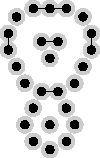
\includegraphics{complex_two.pdf}\\[0.5cm]
    We inflate each point like a balloon and track the radius \\
     setting $r = 0.2$. Can you see the blurry shape?
\end{frame}

\begin{frame}
    \frametitle{
    Simplicial complexes\par\hspace{-0.73cm}
    \small{Spanning the $1$-skeleton}}
    \Fontvi
    \centering
    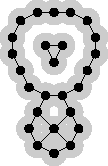
\includegraphics{complex_three.pdf}\\[0.5cm]
    Every time a ball touches another one, we connect them with an edge. \\
    We have $r = 0.4$ and one can already see the sought shape.\\[0.5cm]
\end{frame}

\begin{frame}
    \frametitle{
    Simplicial complexes\par\hspace{-0.73cm}
    \small{Spanning the $1$-skeleton}}
    \Fontvi
    \centering
    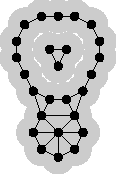
\includegraphics{complex_four.pdf}\\[0.5cm]
    We ommit constructing other simplices than $1$-simplices, \\
    to make the visualization more intuitive. \\
    The result is called $1$-skeleton.
\end{frame}

\begin{frame}
    \frametitle{
    Simplicial complexes\par\hspace{-0.73cm}
    \small{Spanning the $1$-skeleton}}
    \Fontvi
    \centering
    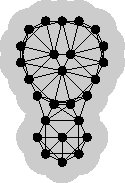
\includegraphics{complex_five.pdf}\\[0.5cm]
    The $1$-skeleton.
\end{frame}

\begin{frame}
    \frametitle{
    Simplicial complexes\par\hspace{-0.73cm}
    \small{Definition}}
    \Fontvi
    Given a set $X = \{x_0, \cdots, x_k\} \subset \mathbb{R}^d$ of $k+1$ points that do not lie on a hyperplane with dimension less than $d$, the $k$-dimensional simplex $\sigma$ spanned by $X$ is the set of convex combinations, such that
    \begin{align}
      \sum_{i=0}^{k} \lambda_i x_i \quad \text{with} \quad \sum_{i=0}^{k} \lambda_i = 1 \quad \text{and} \quad \lambda_i \geq 0.
    \end{align}
\end{frame}

\begin{frame}
    \frametitle{
    Simplicial complexes\par\hspace{-0.73cm}
    \small{Example of a Vietoris-Rips complex}}
    \Fontvi
    \centering
    \begin{tikzpicture}
    \tikzstyle{point}=[circle,thick,draw=black,fill=black,inner sep=0pt,minimum width=4pt,minimum height=4pt]
    \node (a)[point] at (0,0) {};
    \node (b)[point] at (3,0) {};
    \node (c)[point] at (2,2) {};

    \begin{scope}[yshift=2cm]
    \node (d)[point] at (1,1) {};
    \node (e)[point] at (0,2) {};
    \node (f)[point] at (4,2) {};
    \end{scope}

    \node (p)[point,label={[label distance=1cm]5:$P$}] at (1.5,0.5) {};

    \draw[pattern=north east lines] (a.center) -- (p.center) -- (b.center) -- cycle;
    \draw[pattern=north west lines] (a.center) -- (p.center) -- (c.center) -- cycle;
    \draw[pattern=vertical lines]   (b.center) -- (p.center) -- (c.center) -- cycle;
    \draw[pattern=dots] (d.center) -- (e.center) -- (f.center) -- cycle;
    \draw (p.center) -- (d.center);
\end{tikzpicture}\\[0.5cm]
    A simplicial complex composed of seven $0$-faces, \\
    ten $1$-faces, five $2$-faces and one $3$-face.
\end{frame}

\begin{frame}
    \frametitle{
    Simplicial complexes may differ\par\hspace{-0.73cm}
    \small{\v{C}ech vs. Vietoris-Rips complex}}
    \Fontvi
    \centering
    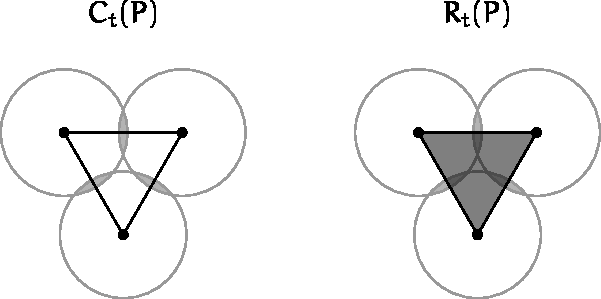
\includegraphics{cechrips.pdf}\\[0.2cm]
    \small{Taken from Tam Thanh Truong: \href{http://bora.uib.no/handle/1956/17245}{Persistent Homology via Quotient Spaces}.}
\end{frame}

\section{Part III: \\ \textbf{Homology groups}}
\begin{frame}
    \frametitle{
    What are we seeking for?\par\hspace{-0.73cm}
    \small{Filtrations of spaces}}
    \Fontvi
    We believe that different data comes from different spaces. How can we detect this and sort the data accordingly?\\[0.5cm]
    \emph{We don't want to distinguish data only by their \textbf{holes}, therefore we introduce a \textbf{magnifying glass} which allows us to capture the \textbf{structure of a topological space} in different granularity.}
\end{frame}

\begin{frame}
    \frametitle{
    Chain groups\par\hspace{-0.73cm}
    \small{Chains and boundaries}}
    \Fontvi
    The \textbf{$k$th chain group} of a \textbf{simplicial complex $K$} is $\langle C_k(K),+ \rangle$, the \textbf{free abelian group} on the oriented $k$-simplices, where $[\sigma] = - [\tau]$ if $\sigma = \tau$ and $\sigma$ and $\tau$ have different orientation. \\[0.5cm]
    An element of $C_k(K)$ is called $k$-chain, $\sum_{i} \lambda_i [\sigma_i], \lambda_i \in \mathbb{Z}, \sigma_i \in K$.
\end{frame}

\begin{frame}
    \frametitle{
    Chain groups\par\hspace{-0.73cm}
    \small{Boundary homomorphism}}
    \Fontvi
    Let $K$ be a simplicial complex and $\sigma \in K$, $\sigma = [v_0,v_1,\cdots,v_k]$. The \textbf{boundary homomorphism} $\delta_k: C_k(K) \rightarrow C_{k-1}(K)$ is
    \begin{align}
        \delta_k \sigma = \sum_{i} (-1)^i [v_0, v_1,\cdots,\hat{v}_i,\cdots,v_n].
    \end{align}
\end{frame}

\begin{frame}
    \frametitle{
    Cycle group and boundary group\par\hspace{-0.73cm}
    \small{Cycles}}
    \Fontvi
    The \textbf{$k$th cycle group $Z_k$} is defined as
    \begin{align}
        Z_k &= \ker \delta_k\\
            &= \{c \in C_k \; | \; \delta_k c = \emptyset\}.
    \end{align}
    An element of this group is called \textbf{$k$-cycle}.
\end{frame}

\begin{frame}
    \frametitle{
    Cycle group and boundary group\par\hspace{-0.73cm}
    \small{Boundaries}}
    \Fontvi
    The \textbf{$k$th boundary group $B_k$} is defined as
    \begin{align}
        B_k &= \text{im}\; \delta_{k+1}\\
            &= \{c \in C_k \; | \; \exists d \in C_{k+1}: c = \delta_{k+1} d\}.
    \end{align}
    An element of this group is called \textbf{$k$-boundary}.
\end{frame}

\begin{frame}
    \frametitle{
    Nested sequences\par\hspace{-0.73cm}
    \small{Following Zomorodian, Edelsbrunner and others}}
    \Fontvi
    \centering
    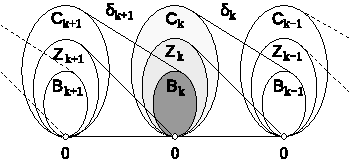
\includegraphics[width=10cm]{relation_of_homs.pdf}\\[0.2cm]
    \small{Taken from Afra Zomorodian: \href{http://graphics.stanford.edu/courses/cs468-04-winter/notes/06.pdf}{Chap. 6, Homology}.}
\end{frame}

\begin{frame}
    \frametitle{
    Boundaries of simplices\par\hspace{-0.73cm}
    \small{Computation of boundaries}}
    \Fontvi
    \centering
    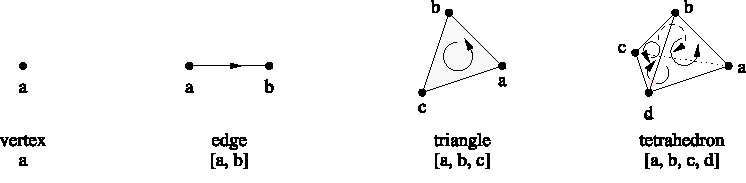
\includegraphics{boundaries.pdf}\\[0.1cm]
    \small{Taken from Afra Zomorodian: \href{http://graphics.stanford.edu/courses/cs468-04-winter/notes/06.pdf}{Chap. 6, Homology}.}\\[0.5cm]
   \begin{enumerate}[leftmargin=3cm]
        \item[edge:] $\delta_1[a,b] = b-a$,
        \item[triangle:] $\delta_2[a,b,c] = [b,c] - [a,c] + [a,b] = [b,c] + [c,a] + [a,b]$,
        \item[tetrahedron:] $\delta_3[a,b,c,d] = [b,c,d] - [a,c,d] + [a,b,d] - [a,b,c]$.
    \end{enumerate}
\end{frame}

\begin{frame}
    \frametitle{
    Chain complex\par\hspace{-0.73cm}}
    \Fontvi
    \centering
    \begin{align}
      0 \xrightarrow[]{\delta_{k+1}} C_k \xrightarrow[]{\delta_{k}} C_{k-1} \xrightarrow[]{\delta_{k-1}} \cdots \xrightarrow[]{\delta_{2}} C_{1} \xrightarrow[]{\delta_{1}} 0
    \end{align}
\end{frame}

\begin{frame}
    \frametitle{
    What are we seeking for?\par\hspace{-0.73cm}
    \small{Filtrations of spaces}}
    \Fontvi
    \centering
    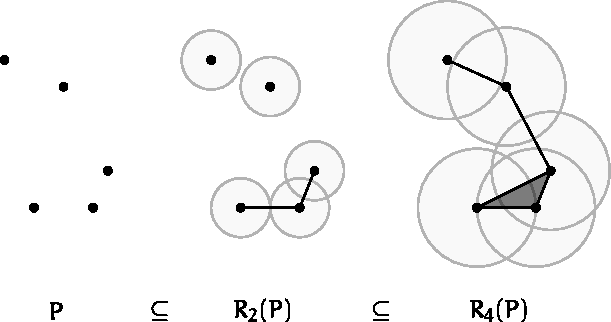
\includegraphics{filtration.pdf}\\[0.2cm]
    \small{Taken from Tam Thanh Truong: \href{http://bora.uib.no/handle/1956/17245}{Persistent Homology via Quotient spaces}.}
\end{frame}

\begin{frame}
    \frametitle{
    Technical details\par\hspace{-0.73cm}}
    \Fontvi
    A \textbf{filtration} is a nested sequence of sets
    \begin{align}
      \emptyset = K_0 \subseteq K_1 \subseteq K_2 \cdots \subseteq K_{k-1} \subseteq K_{k} = K,
    \end{align}
    such that each simplicial complex $K_i$ is a valid subcomplex of $K_{i+1}$. To compute persistent homology is is enough to reduce a \emph{single} boundary matrix of the simplicial complex $K$ in order to get the homology groups along the filtration.
\end{frame}

\begin{frame}
    \frametitle{
    Homology groups\par\hspace{-0.73cm}}
    \Fontvi
    The $k$th \textbf{homology group} of a simplicial complex is defined as
    \begin{align}
      H_k(K) = \ker \delta_k C_k(K) / \text{im}\; \delta_{k+1} C_{k+1}(X).
    \end{align}
    Intuitively, the kernel of the boundary homomorphism of the $k$th chain group gives all $k$-cycles, thus the cycle group, from which we quotient out all elements of the $k$th boundary group, i.e. $H_k(K) = Z_k(K) / B_k(K)$.\\[0.5cm]

    \small{Technical details: Both subgroups, the cycle and boundary group, are normal because our chain groups are abelian.}
\end{frame}

\begin{frame}
    \frametitle{
    Betti numbers\par\hspace{-0.73cm}}
    \Fontvi
    The $k$th \textbf{Betti} number $\beta_k$ is the rank of the $k$th homology group $H_k(K)$ of the topological space $K$.\\[0.5cm]
    \small{We'll track the betti numbers to track the amount of holes along the filtration. Other properties of the vector space could also be helpful.}
\end{frame}

\begin{frame}
    \frametitle{
    Example of Persistent Homology\par\hspace{-0.73cm}
    \small{Persistent homology of a continuous function}}
    \Fontvi
    \centering
    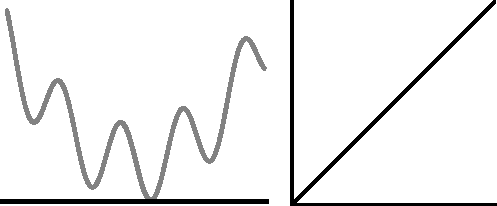
\includegraphics{function_one.pdf}\\[0.2cm]
    \small{Taken from Bastian Rieck: \href{https://bastian.rieck.me/research/talks/an_introduction_to_persistent_homology.pdf}{An Introduction to Persistent Homology}.}
\end{frame}

\begin{frame}
    \frametitle{
    Example of Persistent Homology\par\hspace{-0.73cm}
    \small{Persistent homology of a continuous function}}
    \Fontvi
    \centering
    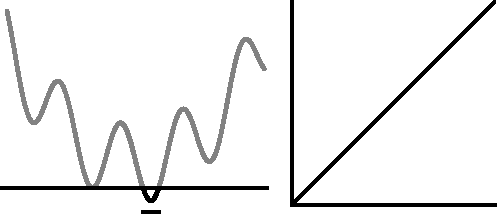
\includegraphics{function_two.pdf}\\[0.2cm]
    \small{Taken from Bastian Rieck: \href{https://bastian.rieck.me/research/talks/an_introduction_to_persistent_homology.pdf}{An Introduction to Persistent Homology}.}
\end{frame}

\begin{frame}
    \frametitle{
    Example of Persistent Homology\par\hspace{-0.73cm}
    \small{Persistent homology of a continuous function}}
    \Fontvi
    \centering
    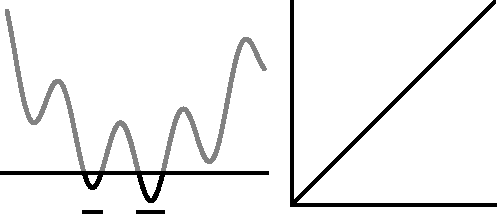
\includegraphics{function_three.pdf}\\[0.2cm]
    \small{Taken from Bastian Rieck: \href{https://bastian.rieck.me/research/talks/an_introduction_to_persistent_homology.pdf}{An Introduction to Persistent Homology}.}
\end{frame}

\begin{frame}
    \frametitle{
    Example of Persistent Homology\par\hspace{-0.73cm}
    \small{Persistent homology of a continuous function}}
    \Fontvi
    \centering
    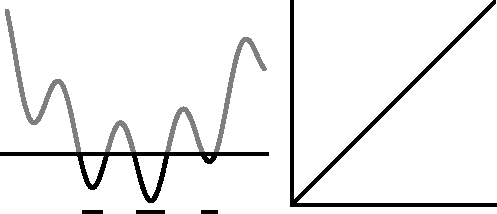
\includegraphics{function_four.pdf}\\[0.2cm]
    \small{Taken from Bastian Rieck: \href{https://bastian.rieck.me/research/talks/an_introduction_to_persistent_homology.pdf}{An Introduction to Persistent Homology}.}
\end{frame}

\begin{frame}
    \frametitle{
    Example of Persistent Homology\par\hspace{-0.73cm}
    \small{Persistent homology of a continuous function}}
    \Fontvi
    \centering
    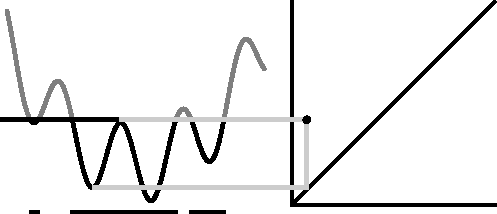
\includegraphics{function_five.pdf}\\[0.2cm]
    \small{Taken from Bastian Rieck: \href{https://bastian.rieck.me/research/talks/an_introduction_to_persistent_homology.pdf}{An Introduction to Persistent Homology}.}
\end{frame}

\begin{frame}
    \frametitle{
    Example of Persistent Homology\par\hspace{-0.73cm}
    \small{Persistent homology of a continuous function}}
    \Fontvi
    \centering
    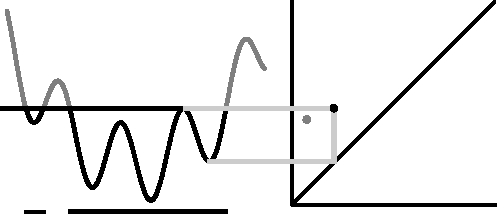
\includegraphics{function_six.pdf}\\[0.2cm]
    \small{Taken from Bastian Rieck: \href{https://bastian.rieck.me/research/talks/an_introduction_to_persistent_homology.pdf}{An Introduction to Persistent Homology}.}
\end{frame}

\begin{frame}
    \frametitle{
    Example of Persistent Homology\par\hspace{-0.73cm}
    \small{Persistent homology of a continuous function}}
    \Fontvi
    \centering
    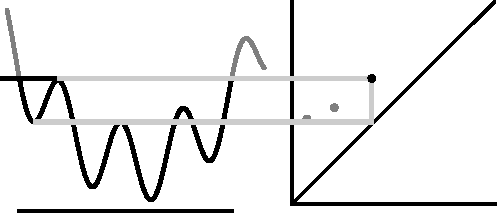
\includegraphics{function_seven.pdf}\\[0.2cm]
    \small{Taken from Bastian Rieck: \href{https://bastian.rieck.me/research/talks/an_introduction_to_persistent_homology.pdf}{An Introduction to Persistent Homology}.}
\end{frame}

\begin{frame}
    \frametitle{
    Example of Persistent Homology\par\hspace{-0.73cm}
    \small{Persistent homology of a continuous function}}
    \Fontvi
    \centering
    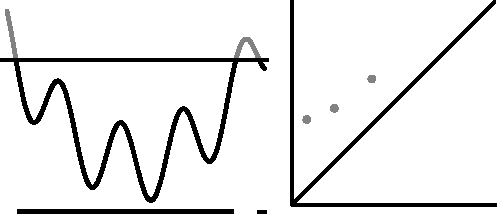
\includegraphics{function_eight.pdf}\\[0.2cm]
    \small{Taken from Bastian Rieck: \href{https://bastian.rieck.me/research/talks/an_introduction_to_persistent_homology.pdf}{An Introduction to Persistent Homology}.}
\end{frame}

\begin{frame}
    \frametitle{
    Example of Persistent Homology\par\hspace{-0.73cm}
    \small{Persistent homology of a continuous function}}
    \Fontvi
    \centering
    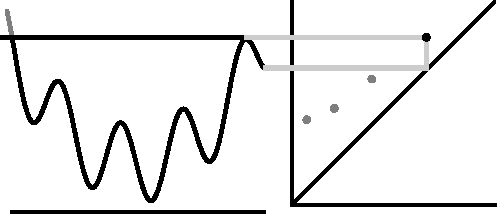
\includegraphics{function_nine.pdf}\\[0.2cm]
    \small{Taken from Bastian Rieck: \href{https://bastian.rieck.me/research/talks/an_introduction_to_persistent_homology.pdf}{An Introduction to Persistent Homology}.}
\end{frame}

\section{Part IV: \\ \textbf{Talks}}
\begin{frame}
    \frametitle{
    Topological spaces and groups\par\hspace{-0.73cm}
    \small{Techies preferred}}
    \Fontvi
    Define and illustrate the concepts topological space, metric space, topology of a metric space, bases and subbases of topologies, continuous mappings and homeomorphisms, compactness, groups, homomorphisms of groups and the most important vector spaces, Hilbert spaces, Banach spaces and Fréchet spaces.\\[0.5cm]
    \small{\textbf{Literature:} Jänich, Klaus. Topologie. Springer-Verlag, 2013. Chap. 1 and 2.}
\end{frame}

\begin{frame}
    \frametitle{
    Simplicial complexes\par\hspace{-0.73cm}
    \small{Techies preferred}}
    \Fontvi
    Define simplicial complexes and simplicial maps. Explain the simplicial approximation theorem and the nerve theorem. You do not need to show the proofs in their entirety here, but you should have worked through them. Sketch the core concepts and ideas.\\[0.5cm]
    \small{
    \textbf{Prerequisites:} Topological spaces and groups\\[0.2cm]
    \textbf{Literature:} James Munkres: Elements of algebraic topology, CRC Press, 2018. Sections $1-3$ and sections $14$ and $16$.}
\end{frame}

\begin{frame}
    \frametitle{
    Simplicial complexes associated with point clouds\par\hspace{-0.73cm}}
    \Fontvi
    Define and show different simplicial complexes on a set of points in a metric space. In particular, show the Voronoi diagrams, the Delaunay complexes, the duality of the two as well as Alpha complexes and Witness complexes.\\[0.5cm]
    \small{\textbf{Prerequisites:} Topological spaces and groups\\[0.2cm]
    \textbf{Literature:} Boissonnat, Jean-Daniel, Frédéric Chazal, and Mariette Yvinec. Geometric and topological inference. Vol. 57. Cambridge University Press, 2018. Chap. 4.2, 4.3, 6.1, 6.2.}
\end{frame}

\begin{frame}
    \frametitle{
    Simplicial and singular homology groups\par\hspace{-0.73cm}
    \small{Techies preferred}}
    \Fontvi
    Explain and define the simplicial homology groups on a simplicial complex, the so-called $\sigma$-complex. Explain what is meant by singular homology and use the cutout theorem to show that the simplicial homology groups match the singular homology groups on a $\sigma$ complex.\\[0.5cm]
    \small{\textbf{Prerequisites:} Topological spaces and groups, Simplicial Complexes\\[0.2cm]
    \textbf{Literature:} Hatcher, Allen. Algebraic topology. Cambridge University Press, 2005. S. 102-106, 128-130.}
\end{frame}

\begin{frame}
    \frametitle{
    Persistent homology\par\hspace{-0.73cm}
    \small{Mathies preferred}}
    \Fontvi
     Define persistent homology, show persistence diagrams and explain persistence  diagrams  using  the  relationship  between  persistent  homology  classes and the critical values of one-dimensional tame functions.  Also explain persis-tent homology on the filtration of point sets in higher-dimensional spaces.\\[0.5cm]
    \small{\textbf{Prerequisites:} Topological spaces and groups, Simplicial Complexes\\[0.2cm]
    \textbf{Literature:} Edelsbrunner, Herbert, and John Harer.  ”Persistent homology-asurvey.” Contemporary mathematics 453 (2008):  257-282.\\
    Boissonnat, Jean-Daniel, Frédéric Chazal, and Mariette Yvinec.  Geometric andtopological inference.  Vol.  57.  Cambridge University Press, 2018.  Chap.  11.5.}
\end{frame}


\begin{frame}
    \frametitle{
    Computation of persistent homology\par\hspace{-0.73cm}
    \small{Mathies preferred}}
    \Fontvi
    Specify the algorithm to calculate persistence diagrams and describe the  matrix  reduction techniques used. Give examples and make exemplary calculations of persistent homology on the triangulation of basic compact geometric objects.\\[0.5cm]
    \small{\textbf{Prerequisites:} Topological spaces and groups, Simplicial Complexes, Simplicial and singular homology groups\\[0.2cm]
    \textbf{Literature:} Afra Zomorodian, and Gunnar Carlsson.  ”Computing persistenthomology.” Discrete \& Computational Geometry 33.2 (2005):  249-274.\\
    Otter, Nina, et al.  ”A roadmap for the computation of persistent homology.”EPJ Data Science 6.1 (2017):  17.}
\end{frame}


\begin{frame}
    \frametitle{
    Persistent homology and cohomology*\par\hspace{-0.73cm}
    \small{Mathies preferred}}
    \Fontvi
    Remind the audience of the definition of persistent homology. Specify the dual concept of persistent cohomology and explain the proof that both persistent homology and persistent cohomology generate the same barcodes. Why is persistent cohomology more efficient to compute?\\[0.5cm]
    \small{\textbf{Prerequisites:} Topological spaces and groups, Simplicial Complexes, Simplicial and singular homology groups, Persistent homology\\[0.2cm]
    \textbf{Literature:} De Silva, Vin, Dmitriy Morozov, and Mikael Vejdemo-Johansson. "Dualities in persistent (co) homology." Inverse Problems 27.12 (2011): 124003.}
\end{frame}


\begin{frame}
    \frametitle{
    Distances and the stability theorem\par\hspace{-0.73cm}}
    \Fontvi
    Describe the stability of the persistence diagrams in relation to the Hausdorff distance, the bottleneck distance and the Wasserstein distance. Give all three metrics and explain them with illustrative examples. Explain the quadrant lemma without formal proof, so that the listener gets a good understanding of the properties of persistence diagrams.\\[0.5cm]
    \small{\textbf{Prerequisites:} Topological spaces and groups, Simplicial Complexes, Simplicial and singular homology groups, Persistent homology\\[0.2cm]
    \textbf{Literature:} David Cohen-Steiner, Herbert Edelsbrunner, and John Harer. "Stability of persistence diagrams." Discrete \& Computational Geometry 37.1 (2007): 103-120.}
\end{frame}

\begin{frame}
    \frametitle{
    Statistics in persistent homology\par\hspace{-0.73cm}}
    \Fontvi
    Define persistence landscapes and make it clear how to obtain them from the persistence diagrams. Explain why the ordinary persistence diagram, unlike the persistence landscape, does not lie in a vector space and explain why this property is important for statistical data analysis.\\[0.5cm]
    \small{\textbf{Prerequisites:} Topological spaces and groups, Simplicial Complexes, Simplicial and singular homology groups, Persistent homology\\[0.2cm]
    \textbf{Literature:} Bubenik, Peter. "Statistical topological data analysis using persistence landscapes." The Journal of Machine Learning Research 16.1 (2015): 77-102.}
\end{frame}

\begin{frame}[plain,noframenumbering]
    \Fontvi
    \centering
    More Questions? \\
    Contact me: {\col luciano.melodia@fau.de}\\
    Thank you for your attention! \\[1cm]
    \begin{tikzpicture}[scale=1.5]

% Saucer
\begin{scope}[shift={(0,-1)}]
    \fill [black!87.5, path fading=fade out] 
      (0,-2/8) ellipse [x radius=6/4, y radius=3/4];
    \shade [left color=gray!20, right color=gray!80] 
      (0,0) ++(180:1.25) arc (180:360:5/4 and 5/8+1/16);
    \shade [left color=gray!40, right color=gray!20] 
      (0,0) ellipse [x radius=5/4, y radius=5/8];
    \shade [right color=gray!40, left color=gray!20] 
      (0,0) ellipse [x radius=5/4/2, y radius=5/8/2];
    \shade [left color=gray!40, right color=gray!20] 
      (0,-1/16) ellipse [x radius=5/4/2-1/16, y radius=5/8/2-1/16];
\end{scope} 

% Handle
\begin{scope}[shift=(10:7/8), rotate=-30, yslant=1/2, xslant=-1/8]
  \shade [top color=gray!80, bottom color=gray!30] 
    (0,0) arc (130:-100:3/8 and 1/2) -- ++(0,1/4) arc (-100:130:1/8 and 1/4) -- cycle;
  \shade [top color=gray!10, bottom color=gray!60] 
    (0,0) arc (130:-100:3/8 and 1/2) -- ++(0,1/32) arc (-100:130:1/4 and 1/3) -- cycle;
\end{scope}

% Cup
\fill [black!75, path fading=fade out] 
    (0,-1) ellipse [x radius=3/4, y radius=1/2];
\shade [left color=gray!60, right color=gray!30] 
  (-1,0) arc (180:360:1 and 5/4);
\shade [bottom color=gray, top color=gray!30, opacity=1/2]
  (-1,0) arc (180:360:1 and 5/4);
\shade [left color=gray!20, right color=gray!40] 
  (0,0) ellipse [x radius=1, y radius=1/2];
\shade [left color=gray!40, right color=gray!20] 
  (0,0) ellipse [x radius=1-1/16, y radius=1/2-1/16];
\shade [bottom color=gray, top color=gray!10, opacity=1/2] 
  (0,0) ellipse [x radius=1-1/16, y radius=1/2-1/16];

% Coffee
\begin{scope}
\clip ellipse [x radius=1-1/16, y radius=1/2-1/16];
\fill [brown!25!black] 
  (0,-1/4) ellipse [x radius=3/4, y radius=3/8];
\fill [brown!50!black, path fading=fade out] 
  (0,-1/4) ellipse [x radius=3/4, y radius=3/8];
\end{scope}

\end{tikzpicture}
\end{frame}
\end{document}
